% answers.tex —— 2009 年·普通高等学校招生考试·上海卷·理科 · 参考答案与详细解析片段
% 由 tools/generate_projects.py 依来源总账自 2009/2009_数学真题_上海理_试题.md + 2009/2009_数学真题_上海理_解析正文.md + 2009/2009_数学真题_上海理_答案要点.md 生成，勿手改（改源 MD 后重跑）


\begin{gktip}
固定候选 PDF 仅含题面，无答案、解析和评分标准，原卷亦未标分值；以下为非官方编者独立推导，官方答案字段为空。题面文字层只作定位，公式、上下标与四幅图（Q4 程序框图、Q5 正四棱柱、Q18 圆与坐标轴、Q19 直三棱柱）均以 300/400 dpi 原页复核后重绘。
\end{gktip}

\begin{answer}
\gksolhead{1}{}

\textbf{题目}：

若复数 $z$ 满足 $z(1+\mathrm i)=1-\mathrm i$（$\mathrm i$ 是虚数单位），则其共轭复数 $\overline z=$\gkblank{}．

\Needspace{4\baselineskip}
\textbf{解析}

\Needspace{5\baselineskip}
由 $z(1+\mathrm i)=1-\mathrm i$：

\nopagebreak[4]
\[z=\frac{1-\mathrm i}{1+\mathrm i}=\frac{(1-\mathrm i)^2}{(1+\mathrm i)(1-\mathrm i)}=\frac{1-2\mathrm i+\mathrm i^2}{2}=\frac{-2\mathrm i}{2}=-\mathrm i .\]

故 $\overline z=\mathrm i$。

\gkanswer{答案：$\mathrm i$。}

\end{answer}
\begin{answer}
\gksolhead{2}{}

\textbf{题目}：

已知集合 $A=\{x\mid x\leqslant1\}$，$B=\{x\mid x\geqslant a\}$，且 $A\cup B=\mathbf R$，则实数 $a$ 的取值范围是\gkblank{}．

\Needspace{4\baselineskip}
\textbf{解析}

$A=(-\infty,1]$，$B=[a,+\infty)$。并集覆盖全体实数，需 $a\leqslant1$。

\gkanswer{答案：$a\leqslant1$。}

\end{answer}
\begin{answer}
\gksolhead{3}{}

\textbf{题目}：

若行列式 $\begin{vmatrix}4&5&x\\1&x&3\\7&8&9\end{vmatrix}$ 中，元素 $4$ 的代数余子式大于 $0$，则 $x$ 满足的条件是\gkblank{}．

\Needspace{4\baselineskip}
\textbf{解析}

\Needspace{5\baselineskip}
元素 $4$ 的代数余子式为

\nopagebreak[4]
\[(-1)^{1+1}\begin{vmatrix}x&3\\8&9\end{vmatrix}=9x-24 .\]

由 $9x-24>0$ 得 $x>\frac83$。

\gkanswer{答案：$x>\frac83$。}

\end{answer}
\begin{answer}
\gksolhead{4}{}

\textbf{题目}：

某算法的程序框图如图所示，则输出量 $y$ 与输入量 $x$ 满足的关系式是\gkblank{}．
\nopagebreak[4]
\begin{center}% 2009 年上海卷理科第 4 题：题图。
% 来源 PDF：普通高考/2009/2009上海理.pdf，SHA256 82ede013bf354097cfc65c1bab2885db813572321b6eb0012f445c1c754d3fa8
% 原页：第 1 页（A3 三栏）第 1 栏，印刷页 553。
% 重绘依据：自上而下「开始」→「输入实数 x」→ 判断「x>1」；是→y←x−2，否→y←2^x；汇合→输出 y→结束；与文科同题一致。
\begin{tikzpicture}[scale=0.95, semithick, >=Stealth,
  node distance=6mm, every node/.style={inner sep=4pt, font=\small}]
  \node (start) [draw, rounded corners=4pt, minimum width=2.2cm, minimum height=0.7cm] {开始};
  \node (input) [draw, trapezium, trapezium left angle=70, trapezium right angle=110,
    minimum width=4.0cm, minimum height=0.8cm, below=of start] {输入实数 $x$};
  \node (cond) [draw, diamond, aspect=2.2, minimum width=4.2cm, minimum height=1.2cm,
    below=of input] {$x>1$};
  \node (yes) [draw, minimum width=2.6cm, minimum height=0.8cm,
    below=of cond, xshift=-2.1cm] {$y\leftarrow x-2$};
  \node (no) [draw, minimum width=2.6cm, minimum height=0.8cm,
    below=of cond, xshift=2.6cm] {$y\leftarrow 2^{x}$};
  \node (output) [draw, trapezium, trapezium left angle=70, trapezium right angle=110,
    minimum width=3.6cm, minimum height=0.8cm, below=of yes, xshift=2.3cm] {输出 $y$};
  \node (end) [draw, rounded corners=4pt, minimum width=2.2cm, minimum height=0.7cm,
    below=of output] {结束};
  \draw[->] (start) -- (input);
  \draw[->] (input) -- (cond);
  \draw[->] (cond) -- node[left, xshift=-1pt] {是} (yes);
  \draw[->] (cond) -- node[above, yshift=1pt] {否} (no);
  \draw[->] (yes) -- (output);
  \draw[->] (no) |- (output);
  \draw[->] (output) -- (end);
\end{tikzpicture}
\end{center}
\nopagebreak[4]
\Needspace{4\baselineskip}
\textbf{解析}

\Needspace{5\baselineskip}
程序框：输入 $x$，判断 $x>1$；成立时 $y\leftarrow x-2$，否则 $y\leftarrow2^x$。故

\nopagebreak[4]
\[y=\begin{cases}x-2,&x>1,\\2^x,&x\leqslant1.\end{cases}\]

\gkanswer{答案：$y=\begin{cases}x-2,&x>1,\\2^x,&x\leqslant1.\end{cases}$}

\end{answer}
\begin{answer}
\gksolhead{5}{}

\textbf{题目}：

如图，若正四棱柱 $ABCD-A_1B_1C_1D_1$ 的底面边长为 $2$，高为 $4$，则异面直线 $BD_1$ 与 $AD$ 所成角的大小是\gkblank{}．（结果用反三角函数表示）
\nopagebreak[4]
\begin{center}% 2009 年上海卷理科第 5 题：题图。
% 来源 PDF：普通高考/2009/2009上海理.pdf，SHA256 82ede013bf354097cfc65c1bab2885db813572321b6eb0012f445c1c754d3fa8
% 原页：第 1 页（A3 三栏）第 1 栏，印刷页 553。
% 重绘依据：正四棱柱底面边长 2、高 4，B-D_1 虚线，AD 为底边；与文科同题一致。
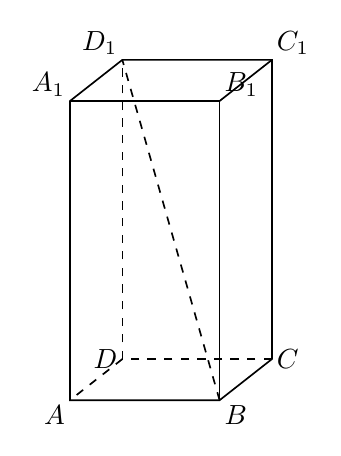
\begin{tikzpicture}[scale=0.95, semithick, every node/.style={inner sep=1.5pt}]
  \coordinate (A)  at (0,0);
  \coordinate (B)  at (2,0);
  \coordinate (D)  at (0.7,0.55);
  \coordinate (C)  at (2.7,0.55);
  \coordinate (A1) at (0,4);
  \coordinate (B1) at (2,4);
  \coordinate (D1) at (0.7,4.55);
  \coordinate (C1) at (2.7,4.55);
  \draw[dashed] (D) -- (D1);
  \draw[dashed] (C) -- (D);
  \draw[dashed] (D) -- (A);
  \draw (A) -- (B) -- (C) -- (C1) -- (D1) -- (A1) -- cycle;
  \draw (A) -- (A1);
  \draw (B) -- (B1);
  \draw (C) -- (C1);
  \draw (B1) -- (C1);
  \draw (A1) -- (B1);
  \draw[dashed] (B) -- (D1);
  \node[anchor=north east] at (A)  {$A$};
  \node[anchor=north west] at (B)  {$B$};
  \node[anchor=west]       at (C)  {$C$};
  \node[anchor=east]       at (D)  {$D$};
  \node[anchor=south east] at (A1) {$A_1$};
  \node[anchor=south west] at (B1) {$B_1$};
  \node[anchor=south west] at (C1) {$C_1$};
  \node[anchor=south east] at (D1) {$D_1$};
\end{tikzpicture}
\end{center}
\nopagebreak[4]
\Needspace{4\baselineskip}
\textbf{解析}

\Needspace{5\baselineskip}
设 $A(0,0,0)$、$B(2,0,0)$、$D(0,2,0)$、$D_1(0,2,4)$，则

\nopagebreak[4]
\[\overrightarrow{BD_1}=(-2,2,4),\qquad \overrightarrow{AD}=(0,2,0).\]

\nopagebreak[4]
\[\cos\theta=\frac{|\overrightarrow{BD_1}\cdot\overrightarrow{AD}|}{|\overrightarrow{BD_1}||\overrightarrow{AD}|}
=\frac{4}{2\sqrt6\cdot2}=\frac{1}{\sqrt6}=\frac{\sqrt6}{6}.\]

故所成角为 $\arccos\frac{\sqrt6}{6}$。

\gkanswer{答案：$\arccos\frac{\sqrt6}{6}$。}

\end{answer}
\begin{answer}
\gksolhead{6}{}

\textbf{题目}：

函数 $y=2\cos^2x+\sin2x$ 的最小值是\gkblank{}．

\Needspace{4\baselineskip}
\textbf{解析}

\nopagebreak[4]
\[y=2\cos^2x+\sin2x=1+\cos2x+\sin2x=1+\sqrt2\sin\left(2x+\frac\pi4\right),\]

最小值为 $1-\sqrt2$。

\gkanswer{答案：$1-\sqrt2$。}

\end{answer}
\begin{answer}
\gksolhead{7}{}

\textbf{题目}：

某学校要从 $5$ 名男生和 $2$ 名女生中选出 $2$ 人作为上海世博会志愿者，若用随机变量 $\xi$ 表示选出的志愿者中女生的人数，则数学期望 $E\xi=$\gkblank{}．（结果用最简分数表示）

\Needspace{4\baselineskip}
\textbf{解析}

\Needspace{5\baselineskip}
从 $7$ 人中选 $2$ 人，共 $\mathrm C_7^2=21$ 种。$\xi$ 为女生人数：

\nopagebreak[4]
\[P(\xi=0)=\frac{\mathrm C_5^2}{21}=\frac{10}{21},\quad
P(\xi=1)=\frac{5\cdot2}{21}=\frac{10}{21},\quad
P(\xi=2)=\frac{\mathrm C_2^2}{21}=\frac1{21}.\]

\nopagebreak[4]
\[E\xi=0\cdot\frac{10}{21}+1\cdot\frac{10}{21}+2\cdot\frac1{21}=\frac{12}{21}=\frac47 .\]

\gkanswer{答案：$\frac47$。}

\end{answer}
\begin{answer}
\gksolhead{8}{}

\textbf{题目}：

已知三个球的半径 $R_1,R_2,R_3$ 满足 $R_1+2R_2=3R_3$，则它们的表面积 $S_1,S_2,S_3$ 满足的等量关系是\gkblank{}．

\Needspace{4\baselineskip}
\textbf{解析}

\Needspace{5\baselineskip}
$S_i=4\pi R_i^2$，故 $R_i=\frac{\sqrt{S_i}}{2\sqrt\pi}$。代入 $R_1+2R_2=3R_3$：

\nopagebreak[4]
\[\frac{\sqrt{S_1}}{2\sqrt\pi}+2\cdot\frac{\sqrt{S_2}}{2\sqrt\pi}=3\cdot\frac{\sqrt{S_3}}{2\sqrt\pi},\]

\Needspace{5\baselineskip}
即

\nopagebreak[4]
\[\sqrt{S_1}+2\sqrt{S_2}=3\sqrt{S_3}.\]

\gkanswer{答案：$\sqrt{S_1}+2\sqrt{S_2}=3\sqrt{S_3}$。}

\end{answer}
\begin{answer}
\gksolhead{9}{}

\textbf{题目}：

已知 $F_1$、$F_2$ 是椭圆 $C:\dfrac{x^2}{a^2}+\dfrac{y^2}{b^2}=1$（$a>b>0$）的两个焦点，$P$ 为椭圆 $C$ 上一点，且 $\overrightarrow{PF_1}\perp\overrightarrow{PF_2}$．若 $\triangle PF_1F_2$ 的面积为 $9$，则 $b=$\gkblank{}．

\Needspace{4\baselineskip}
\textbf{解析}

\Needspace{5\baselineskip}
设 $|PF_1|=m$、$|PF_2|=n$。由 $\overrightarrow{PF_1}\perp\overrightarrow{PF_2}$ 得 $m^2+n^2=4c^2$；由椭圆定义 $m+n=2a$，故

\nopagebreak[4]
\[mn=\frac{(m+n)^2-(m^2+n^2)}{2}=\frac{4a^2-4c^2}{2}=2b^2 .\]

\Needspace{5\baselineskip}
面积

\nopagebreak[4]
\[\frac12mn=b^2=9\ \Longrightarrow\ b=3 .\]

\gkanswer{答案：$3$。}

\end{answer}
\begin{answer}
\gksolhead{10}{}

\textbf{题目}：

在极坐标系中，由三条直线 $\theta=0$，$\theta=\dfrac{\pi}{3}$，$\rho\cos\theta+\rho\sin\theta=1$ 围成图形的面积是\gkblank{}．

\Needspace{4\baselineskip}
\textbf{解析}

$\theta=0$ 为 $x$ 轴，$\theta=\frac\pi3$ 为射线 $y=\sqrt3x$，$\rho\cos\theta+\rho\sin\theta=1$ 为 $x+y=1$。

\Needspace{5\baselineskip}
三角形顶点为 $(0,0)$、$(1,0)$ 与 $y=\sqrt3x$、$x+y=1$ 的交点 $\left(\frac{1}{1+\sqrt3},\frac{\sqrt3}{1+\sqrt3}\right)$。面积

\nopagebreak[4]
\[S=\frac12\cdot1\cdot\frac{\sqrt3}{1+\sqrt3}=\frac{\sqrt3}{2(1+\sqrt3)}=\frac{3-\sqrt3}{4}.\]

\gkanswer{答案：$\frac{3-\sqrt3}{4}$。}

\end{answer}
\begin{answer}
\gksolhead{11}{}

\textbf{题目}：

当 $0\leqslant x\leqslant1$，不等式 $\sin\dfrac{\pi x}{2}\geqslant kx$ 成立，则实数 $k$ 的取值范围是\gkblank{}．

\Needspace{4\baselineskip}
\textbf{解析}

\Needspace{5\baselineskip}
$x=0$ 时 $0\geqslant0$ 成立。$x>0$ 时需

\nopagebreak[4]
\[k\leqslant\frac{\sin\frac{\pi x}{2}}{x}.\]

\Needspace{5\baselineskip}
令 $u=\frac{\pi x}{2}\in\left(0,\frac\pi2\right]$，则

\nopagebreak[4]
\[\frac{\sin\frac{\pi x}{2}}{x}=\frac\pi2\cdot\frac{\sin u}{u}.\]

\Needspace{5\baselineskip}
考察 $\frac{\sin u}{u}$：

\nopagebreak[4]
\[\left(\frac{\sin u}{u}\right)'=\frac{u\cos u-\sin u}{u^2}<0\]

\Needspace{5\baselineskip}
（因 $\tan u>u$），故 $\frac{\sin u}{u}$ 在 $\left(0,\frac\pi2\right]$ 上递减，最小值在 $u=\frac\pi2$ 处为 $\frac{2}{\pi}$。于是原式最小值为

\nopagebreak[4]
\[\frac\pi2\cdot\frac2\pi=1 .\]

故 $k\leqslant1$。

\gkanswer{答案：$k\leqslant1$。}

\end{answer}
\begin{answer}
\gksolhead{12}{}

\textbf{题目}：

已知函数 $f(x)=\sin x+\tan x$．项数为 $27$ 的等差数列 $\{a_n\}$ 满足 $a_n\in\left(-\dfrac{\pi}{2},\dfrac{\pi}{2}\right)$，且公差 $d\neq0$．若 $f(a_1)+f(a_2)+\cdots+f(a_{27})=0$，则当 $k=$\gkblank{}时，$f(a_k)=0$．

\Needspace{4\baselineskip}
\textbf{解析}

同上海文第 13 题。$f(x)=\sin x+\tan x$ 在 $\left(-\frac\pi2,\frac\pi2\right)$ 上为奇函数且严格递增；27 项等差数列中项为 $a_{14}$，各项关于 $a_{14}$ 对称。若中项为 $0$，则 $f(a_i)+f(a_{28-i})=0$，总和为 $0$；反之总和为 $0$ 迫使 $a_{14}=0$。故 $f(a_{14})=0$，$k=14$。

\gkanswer{答案：$14$。}

\end{answer}
\begin{answer}
\gksolhead{13}{}

\textbf{题目}：

某地街道呈现东—西、南—北向的网格状，相邻街距都为 $1$，两街道相交的点称为格点．若以互相垂直的两条街道为轴建立直角坐标系，现有下述格点 $(-2,2)$，$(3,1)$，$(3,4)$，$(-2,3)$，$(4,5)$，$(6,6)$ 为报刊零售点．请确定一个格点（除零售点外）\gkblank{}为发行站，使 $6$ 个零售点沿街道到发行站之间路程的和最短．

\Needspace{4\baselineskip}
\textbf{解析}

路程为曼哈顿距离，$x$、$y$ 方向独立。

\Needspace{5\baselineskip}
横坐标 $-2,-2,3,3,4,6$ 的中位区间为 $[3,3]$；纵坐标 $1,2,3,4,5,6$ 的中位区间为 $[3,4]$。最优格点为 $(3,3)$ 或 $(3,4)$，其中 $(3,4)$ 是零售点，须排除。故取

\nopagebreak[4]
\[(3,3).\]

（核对总路程：$6+2+1+5+3+6=23$。）

\gkanswer{答案：$(3,3)$。}

\end{answer}
\begin{answer}
\gksolhead{14}{}

\textbf{题目}：

将函数 $y=\sqrt{4+6x-x^2}-2$（$x\in[0,6]$）的图象绕坐标原点逆时针方向旋转角 $\theta$（$0\leqslant\theta\leqslant\alpha$），得到曲线 $C$．若对于每一个旋转角 $\theta$，曲线 $C$ 都是一个函数的图象，则 $\alpha$ 的最大值为\gkblank{}．

\Needspace{4\baselineskip}
\textbf{解析}

\nopagebreak[4]
\[y=\sqrt{4+6x-x^2}-2\ \Longrightarrow\ y+2=\sqrt{13-(x-3)^2},\]

故曲线是圆 $(x-3)^2+(y+2)^2=13$ 的上弧，端点 $(0,0)$、$(6,0)$。

\Needspace{5\baselineskip}
端点处切线斜率：由隐函数求导

\nopagebreak[4]
\[2(x-3)+2(y+2)y'=0\ \Longrightarrow\ y'=-\frac{x-3}{y+2}.\]

\Needspace{5\baselineskip}
在 $(0,0)$ 处 $y'=\frac32$，在 $(6,0)$ 处 $y'=-\frac32$。切线倾角范围为

\nopagebreak[4]
\[\left[-\arctan\frac32,\ \arctan\frac32\right].\]

\Needspace{5\baselineskip}
逆时针旋转 $\theta$ 后，倾角范围变为 $\left[\theta-\arctan\frac32,\theta+\arctan\frac32\right]$。曲线仍为函数图象需整段切线不越过竖直方向（正上方切线角不超过 $90^\circ$）：

\nopagebreak[4]
\[\theta+\arctan\frac32\leqslant\frac\pi2 .\]

\Needspace{5\baselineskip}
故

\nopagebreak[4]
\[\alpha_{\max}=\frac\pi2-\arctan\frac32=\arctan\frac23 .\]

\gkanswer{答案：$\arctan\frac23$。}

\end{answer}
\begin{answer}
\gksolhead{15}{}

\textbf{题目}：

「$-2\leqslant a\leqslant2$」是「实系数一元二次方程 $x^2+ax+1=0$ 有虚根」的（　）

（A）必要不充分条件

（B）充分不必要条件

（C）充要条件

（D）既不充分也不必要条件

\Needspace{4\baselineskip}
\textbf{解析}

方程有虚根 $\iff$ 判别式 $\Delta=a^2-4<0\iff-2<a<2$。

条件 $-2\leqslant a\leqslant2$ 包含 $(-2,2)$，故由「有虚根」可推出该条件；但 $a=\pm2$ 时方程有实根，条件成立而不满足结论。所以是必要不充分条件，选 A。

\gkanswer{答案：A。}

\end{answer}
\begin{answer}
\gksolhead{16}{}

\textbf{题目}：

若事件 $E$ 与 $F$ 相互独立，且 $P(E)=P(F)=\dfrac14$，则 $P(E\cap F)$ 的值等于（　）

（A）$0$

（B）$\dfrac1{16}$

（C）$\dfrac14$

（D）$\dfrac12$

\Needspace{4\baselineskip}
\textbf{解析}

\Needspace{5\baselineskip}
$E$、$F$ 独立，故

\nopagebreak[4]
\[P(E\cap F)=P(E)P(F)=\frac14\cdot\frac14=\frac1{16},\]

选 B。

\gkanswer{答案：B。}

\end{answer}
\begin{answer}
\gksolhead{17}{}

\textbf{题目}：

在发生某公共卫生事件期间，有专业机构认为该事件在一段时间没有发生在规模群体感染的标志为「连续 $10$ 天，每天新增疑似病例不超过 $7$ 人」．根据过去 $10$ 天甲、乙、丙、丁四地新增疑似病例数据，一定符合该标志的是（　）

（A）甲地：总体均值为 $3$，中位数为 $4$

（B）乙地：总体均值为 $1$，总体方差大于 $0$

（C）丙地：中位数为 $2$，众数为 $3$

（D）丁地：总体均值为 $2$，总体方差为 $3$

\Needspace{4\baselineskip}
\textbf{解析}

同上海文第 18 题。丁地均值 $2$、方差 $3$：若某天 $\geqslant8$，该天偏差平方 $(8-2)^2=36$，而 $10$ 天偏差平方和为 $10\times3=30$，矛盾。故丁地每天都不超过 $7$，选 D。

\gkanswer{答案：D。}

\end{answer}
\begin{answer}
\gksolhead{18}{}

\textbf{题目}：

过圆 $C:(x-1)^2+(y-1)^2=1$ 的圆心，作直线分别交 $x$、$y$ 正半轴于点 $A$、$B$，$\triangle AOB$ 被圆分成四部分（如图），若这四部分图形面积满足 $S_{\mathrm I}+S_{\mathrm{IV}}=S_{\mathrm{II}}+S_{\mathrm{III}}$，则直线 $AB$ 有（　）
\nopagebreak[4]
\begin{center}% 2009 年上海卷理科第 18 题：过圆 C 圆心的直线交 x、y 正半轴于 A、B，圆把三角形分成四部分。
% 来源 PDF：普通高考/2009/2009上海理.pdf，SHA256 82ede013bf354097cfc65c1bab2885db813572321b6eb0012f445c1c754d3fa8
% 原页：第 1 页（A3 三栏）第 2 栏下部，印刷页 553，图在题干下方。
% 重绘依据：x、y 轴正方向，圆心 C(1,1)、半径 1（与两轴相切）；直线过 C 交 x 轴于 A、y 轴于 B，
%   取 A 在右、B 在上；四个区域标 I（近 A）、II（近 O）、III（近 B）、IV（圆内 C 附近）。
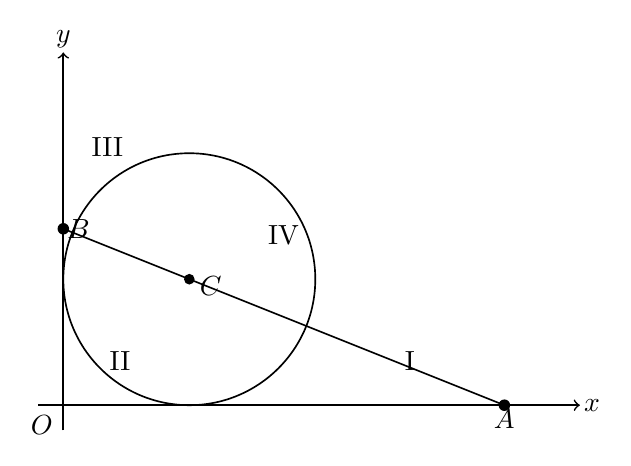
\begin{tikzpicture}[scale=1.6, semithick, every node/.style={inner sep=1.2pt}]
  \draw[->] (-0.2,0) -- (4.1,0) node[anchor=west] {$x$};
  \draw[->] (0,-0.2) -- (0,2.8) node[anchor=south] {$y$};
  \node[anchor=north east] at (-0.05,-0.05) {$O$};
  \draw (1,1) circle (1);
  \fill (1,1) circle (1.2pt);
  \node[anchor=north west] at (1.05,1.05) {$C$};
  \coordinate (A) at (3.5,0);
  \coordinate (B) at (0,1.4);
  \draw (A) -- (B);
  \fill (A) circle (1.3pt) node[anchor=north] {$A$};
  \fill (B) circle (1.3pt) node[anchor=west] {$B$};
  \node at (2.75,0.35) {$\mathrm I$};
  \node at (0.45,0.35) {$\mathrm{II}$};
  \node at (0.35,2.05) {$\mathrm{III}$};
  \node at (1.75,1.35) {$\mathrm{IV}$};
\end{tikzpicture}
\end{center}
\nopagebreak[4]
（A）$0$ 条

（B）$1$ 条

（C）$2$ 条

（D）$3$ 条

\Needspace{4\baselineskip}
\textbf{解析}

\Needspace{5\baselineskip}
设 $\angle BAO=x\in\left(0,\frac\pi2\right)$。令

\nopagebreak[4]
\[f(x)=(S_{\mathrm I}+S_{\mathrm{IV}})-(S_{\mathrm{II}}+S_{\mathrm{III}}).\]

当 $x$ 增大（直线 $AB$ 顺时针旋转）时，$\triangle AOB$ 的形状随之变化：$S_{\mathrm I}+S_{\mathrm{IV}}$ 单调递减，而 $S_{\mathrm{II}}+S_{\mathrm{III}}$ 单调递增，故 $f$ 严格递减且连续。

当 $x\to0^+$ 时直线趋近于 $y$ 轴，$S_{\mathrm I}+S_{\mathrm{IV}}$ 较大，$f>0$；当 $x\to\frac\pi2^-$ 时直线趋近于 $x$ 轴，$S_{\mathrm I}+S_{\mathrm{IV}}$ 较小，$f<0$。

由零点定理与严格单调性，$f(x)=0$ 在 $\left(0,\frac\pi2\right)$ 内恰有一个解。故这样的直线有且仅有 $1$ 条，选 B。

\gkanswer{答案：B（$1$ 条）。}

\end{answer}
\begin{answer}
\gksolhead{19}{}

\textbf{题目}：

如图，在直三棱柱 $ABC-A_1B_1C_1$ 中，$AA_1=BC=AB=2$，$AB\perp BC$，求二面角 $B_1-A_1C-C_1$ 的大小．
\nopagebreak[4]
\begin{center}% 2009 年上海卷理科第 19 题：直三棱柱 ABC-A_1B_1C_1，AA_1=BC=AB=2，AB⊥BC。
% 来源 PDF：普通高考/2009/2009上海理.pdf，SHA256 82ede013bf354097cfc65c1bab2885db813572321b6eb0012f445c1c754d3fa8
% 原页：第 2 页（A3 三栏）第 1 栏上部，印刷页 554，图在题干下方。
% 重绘依据：底面直角三角形 AB⊥BC，B 在右下、A 在左下、C 在右后；
%   侧棱竖直，上底同名加下标 1；A_1C、B_1C 为二面角相关线，AC 被遮挡画虚线。
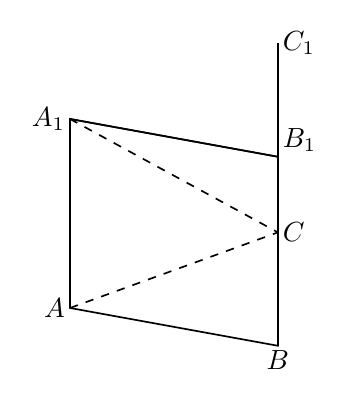
\begin{tikzpicture}[scale=1.2, semithick, every node/.style={inner sep=1.5pt}]
  \coordinate (A)  at (0,0.4);
  \coordinate (B)  at (2.2,0);
  \coordinate (C)  at (2.2,1.2);
  \coordinate (A1) at (0,2.4);
  \coordinate (B1) at (2.2,2.0);
  \coordinate (C1) at (2.2,3.2);
  % 被遮的底边 AC
  \draw[dashed] (A) -- (C);
  % 可见棱
  \draw (A) -- (B) -- (C) -- (C1) -- (B1) -- (A1) -- cycle;
  \draw (B) -- (B1);
  \draw (C) -- (C1);
  \draw (A1) -- (B1);
  \draw (B1) -- (C1);
  % 二面角相关线
  \draw[dashed] (A1) -- (C);
  \draw (B1) -- (C);
  % 标注
  \node[anchor=east] at (A) {$A$};
  \node[anchor=north] at (B) {$B$};
  \node[anchor=west] at (C) {$C$};
  \node[anchor=east] at (A1) {$A_1$};
  \node[anchor=south west] at (B1) {$B_1$};
  \node[anchor=west] at (C1) {$C_1$};
\end{tikzpicture}
\end{center}
\nopagebreak[4]
\Needspace{4\baselineskip}
\textbf{解析}

\Needspace{5\baselineskip}
由 $AB\perp BC$、$BC=AB=2$、$AA_1=2$，设

\nopagebreak[4]
\[B(0,0,0),\quad A(2,0,0),\quad C(0,2,0),\]
\nopagebreak[4]
\[A_1(2,0,2),\quad B_1(0,0,2),\quad C_1(0,2,2).\]

\Needspace{5\baselineskip}
平面 $A_1CC_1$ 的法向量

\nopagebreak[4]
\[\mathbf n_1=\overrightarrow{CA_1}\times\overrightarrow{CC_1}=(2,-2,2)\times(0,0,2)=(-4,-4,0),\]

取 $(1,1,0)$。

\Needspace{5\baselineskip}
平面 $B_1A_1C$ 的法向量

\nopagebreak[4]
\[\mathbf n_2=\overrightarrow{A_1B_1}\times\overrightarrow{A_1C}=(-2,0,0)\times(-2,2,-2)=(0,-4,-4),\]

\Needspace{5\baselineskip}
取 $(0,1,1)$。于是

\nopagebreak[4]
\[\cos\theta=\frac{|\mathbf n_1\cdot\mathbf n_2|}{|\mathbf n_1||\mathbf n_2|}
=\frac{1}{\sqrt2\cdot\sqrt2}=\frac12 .\]

故二面角 $B_1-A_1C-C_1$ 为 $\frac\pi3$（方向核对：半平面取向给出锐角）。

\gkanswer{答案：$\frac{\pi}{3}$。}

\end{answer}
\begin{answer}
\gksolhead{20}{}

\textbf{题目}：

\Needspace{5\baselineskip}
有时可用函数

\nopagebreak[4]
\[f(x)=\begin{cases}0.1+15\ln\dfrac{a}{a-x},&x\leqslant6,\\[6pt] \dfrac{x-4.4}{x-4},&x>6,\end{cases}\]

描述学习某学科知识的掌握程度，其中 $x$ 表示某学科知识的学习次数（$x\in\mathbf N^*$），$f(x)$ 表示对该学科知识的掌握程度，正实数 $a$ 与学科知识有关．

（1）证明：当 $x\geqslant7$ 时，掌握程度的增加量 $f(x+1)-f(x)$ 总是下降；

（2）根据经验，学科甲、乙、丙对应的 $a$ 的取值区间分别为 $(115,121]$、$(121,127]$、$(121,133]$．当学习某学科知识 $6$ 次时，掌握程度是 $85\%$，请确定相应的学科．

\Needspace{4\baselineskip}
\textbf{解析}

\Needspace{5\baselineskip}
（1）$x\geqslant7$ 时 $f(x)=\frac{x-4.4}{x-4}=1-\frac{0.4}{x-4}$，故

\nopagebreak[4]
\[f(x+1)-f(x)=-\frac{0.4}{(x-3)(x-4)} .\]

其绝对值 $\frac{0.4}{(x-3)(x-4)}$ 随 $x$ 增大而减小，故增加量总是下降。

\Needspace{5\baselineskip}
（2）$x=6$ 时用第一段：

\nopagebreak[4]
\[0.1+15\ln\frac{a}{a-6}=0.85\ \Longrightarrow\ \ln\frac{a}{a-6}=0.05,\]

\nopagebreak[4]
\[a=\frac{6\mathrm e^{0.05}}{\mathrm e^{0.05}-1}=\frac{6}{1-\mathrm e^{-0.05}}\approx123.03 .\]

$123.03\in(121,127]$，故对应学科乙。

\begin{gktip}
源疑点：原页把丙的区间印作 $(121,133]$，与乙 $(121,127]$ 重叠，$123.03$ 同时落入两区间；按三区间应互斥的通常意图（丙应为 $(127,133]$），判定为乙。照录原页区间，登记 ISSUE。
\end{gktip}

\gkanswer{答案：（1）证明见解析；（2）学科乙。}

\end{answer}
\begin{answer}
\gksolhead{21}{}

\textbf{题目}：

已知双曲线 $C:\dfrac{x^2}{2}-y^2=1$，设过点 $A(-3\sqrt2,0)$ 的直线 $l$ 的方向向量 $\boldsymbol e=(1,k)$．

（1）当直线 $l$ 与双曲线 $C$ 的一条渐近线 $m$ 平行时，求直线 $l$ 的方程及 $l$ 与 $m$ 的距离；

（2）证明：当 $k>\dfrac{\sqrt2}{2}$ 时，在双曲线 $C$ 的右支上不存在点 $Q$，使之到直线 $l$ 的距离为 $\sqrt6$．

\Needspace{4\baselineskip}
\textbf{解析}

\Needspace{5\baselineskip}
（1）双曲线 $\frac{x^2}{2}-y^2=1$ 的渐近线为 $y=\pm\frac{x}{\sqrt2}$。$l$ 与渐近线平行，故 $k=\pm\frac{1}{\sqrt2}$。过 $A(-3\sqrt2,0)$：

\nopagebreak[4]
\[l:y=\pm\frac{x+3\sqrt2}{\sqrt2}.\]

\Needspace{5\baselineskip}
取 $k=\frac{1}{\sqrt2}$，$l:x-\sqrt2y+3\sqrt2=0$，$m:x-\sqrt2y=0$，距离

\nopagebreak[4]
\[d=\frac{|3\sqrt2|}{\sqrt{1+2}}=\sqrt6 .\]

$k=-\frac{1}{\sqrt2}$ 同理。

\Needspace{5\baselineskip}
（2）同上海文第 22(3)。对右支上 $Q(x,y)$，$x\geqslant\sqrt2$，$|y|<\frac{x}{\sqrt2}$；当 $k>\frac{\sqrt2}{2}$ 时

\nopagebreak[4]
\[kx-y\geqslant kx-|y|>\left(k-\frac1{\sqrt2}\right)x\geqslant0,\]

\Needspace{5\baselineskip}
故

\nopagebreak[4]
\[d(Q,l)\geqslant\frac{3\sqrt2k}{\sqrt{1+k^2}}
=\frac{3\sqrt2}{\sqrt{1+1/k^2}}>\frac{3\sqrt2}{\sqrt3}=\sqrt6 .\]

故不存在到 $l$ 距离为 $\sqrt6$ 的点。

\gkanswer{答案：（1）$l:y=\pm\frac{x+3\sqrt2}{\sqrt2}$，距离 $\sqrt6$；（2）证明见解析。}

\end{answer}
\begin{answer}
\gksolhead{22}{}

\textbf{题目}：

已知函数 $y=f^{-1}(x)$ 是 $y=f(x)$ 的反函数．定义：若对给定的实数 $a$（$a\neq0$），函数 $y=f(x+a)$ 与 $y=f^{-1}(x+a)$ 互为反函数，则称 $y=f(x)$ 满足「$a$ 和性质」；若函数 $y=f(ax)$ 与 $y=f^{-1}(ax)$ 互为反函数，则称 $y=f(x)$ 满足「$a$ 积性质」．

（1）判断函数 $g(x)=x^2$（$x>0$）是否满足「$1$ 和性质」，并说明理由；

（2）求所有满足「$2$ 和性质」的一次函数；

（3）设函数 $y=f(x)$（$x>0$）对任何 $a>0$，满足「$a$ 积性质」，求 $y=f(x)$ 的表达式．

\Needspace{4\baselineskip}
\textbf{解析}

\Needspace{5\baselineskip}
（1）$g(x+1)=(x+1)^2$（$x>0$），其反函数为 $y=\sqrt x-1$（$x>1$）；而

\nopagebreak[4]
\[g^{-1}(x+1)=\sqrt{x+1}.\]

二者不相等，故 $g$ 不满足「$1$ 和性质」。

\Needspace{5\baselineskip}
（2）设 $f(x)=kx+b$（$k\neq0$）。$f(x+2)=kx+2k+b$，反函数为

\nopagebreak[4]
\[y=\frac{x-2k-b}{k}.\]

\Needspace{5\baselineskip}
而 $f^{-1}(x+2)=\frac{x+2-b}{k}$。恒等要求

\nopagebreak[4]
\[-2-\frac bk=\frac{2-b}{k}\ \Longrightarrow\ -2k-b=2-b\ \Longrightarrow\ k=-1 .\]

故 $f(x)=-x+b$（$b$ 任意）。

\Needspace{5\baselineskip}
（3）设 $h=f^{-1}$。$y=f(ax)$ 的反函数为 $y=\frac1a h(x)$，条件给出

\nopagebreak[4]
\[h(ax)=\frac1a h(x)\quad(a>0,\ x>0).\]

\Needspace{5\baselineskip}
令 $x=1$ 得 $h(a)=\frac{h(1)}{a}$，故 $h(x)=\frac cx$（$c=h(1)\neq0$）。于是

\nopagebreak[4]
\[f(x)=h^{-1}(x)=\frac cx\quad(c\neq0).\]

\begin{gktip}
说明：题设只推出 $f(x)=c/x$（$c\neq0$），$c$ 未被唯一确定；$f(x)=1/x$ 只是其中一例，需额外的归一化条件才能定出。
\end{gktip}

\gkanswer{答案：（1）不满足；（2）$f(x)=-x+b$（$b$ 任意）；（3）$f(x)=\frac cx$（$c\neq0$）。}

\end{answer}
\begin{answer}
\gksolhead{23}{}

\textbf{题目}：

已知 $\{a_n\}$ 是公差为 $d$ 的等差数列，$\{b_n\}$ 是公比为 $q$ 的等比数列．

（1）若 $a_n=3n+1$，是否存在 $m$、$k\in\mathbf N^*$，有 $a_m+a_{m+1}=a_k$？请说明理由；

（2）找出所有数列 $\{a_n\}$ 和 $\{b_n\}$，使对一切 $n\in\mathbf N^*$，$\dfrac{a_{n+1}}{a_n}=b_n$，并说明理由；

（3）若 $a_1=5$，$d=4$，$b_1=q=3$，试确定所有的 $p$，使数列 $\{a_n\}$ 中存在某个连续 $p$ 项的和是数列 $\{b_n\}$ 中的一项，请证明．

\Needspace{4\baselineskip}
\textbf{解析}

（1）$a_m+a_{m+1}=(3m+1)+(3m+4)=6m+5$。若 $=3k+1$，则 $k=2m+\frac43\notin\mathbf N^*$，故不存在。

\Needspace{5\baselineskip}
（2）由 $\frac{a_{n+1}}{a_n}=b_n$。若 $d\neq0$，则

\nopagebreak[4]
\[\frac{a_{n+1}}{a_n}=1+\frac{d}{a_1+(n-1)d},\]

它关于 $n$ 单调且趋于 $1$，不是等比数列，故 $d=0$。此时 $a_n=c$（$c\neq0$），$b_n=1$，是首项与公比均为 $1$ 的等比数列。

\Needspace{5\baselineskip}
（3）$a_n=4n+1$，$b_n=3^n$。连续 $p$ 项（从 $a_{m+1}$ 起）之和

\nopagebreak[4]
\[S=p(4m+2p-1).\]

\Needspace{5\baselineskip}
若 $S=3^k$，则 $p\mid3^k$，故 $p=3^j$。反之，当 $p=3^j$ 时，取 $k-j$ 为偶数且足够大，令

\nopagebreak[4]
\[4m+2p-1=3^{k-j}.\]

\Needspace{5\baselineskip}
右边 $\equiv1\pmod4$，而 $2p-1=2\cdot3^j-1\equiv1\pmod4$，故

\nopagebreak[4]
\[m=\frac{3^{k-j}-2\cdot3^j+1}{4}\]

为正整数。于是 $S=3^j\cdot3^{k-j}=3^k=b_k$。

故所有 $p=3^j$（$j=0,1,2,\cdots$）满足要求。

\gkanswer{答案：（1）不存在；（2）$a_n=c$（$c\neq0$ 常数），$b_n=1$；（3）所有 $p=3^j$（$j=0,1,2,\cdots$）。}

\end{answer}